\chapter{Architettura di Sistema}\label{cap:Architettura}

%\begin{minipage}{12cm}\textit{Se lo si desidera, utilizzare questo spazio per inserire un breve riassunto di ci\`o che verr\`a detto in questo capitolo. Inserire solo i punti salienti.}
%\end{minipage}

%\vspace*{1cm}

\section{Architettura ad alto livello}
Il progetto finale ha come obiettivo la realizzazione di un architettura di controllo per le bobine poloidali presenti nei reattori tokamak.

\begin{figure}[h]
	\centering
	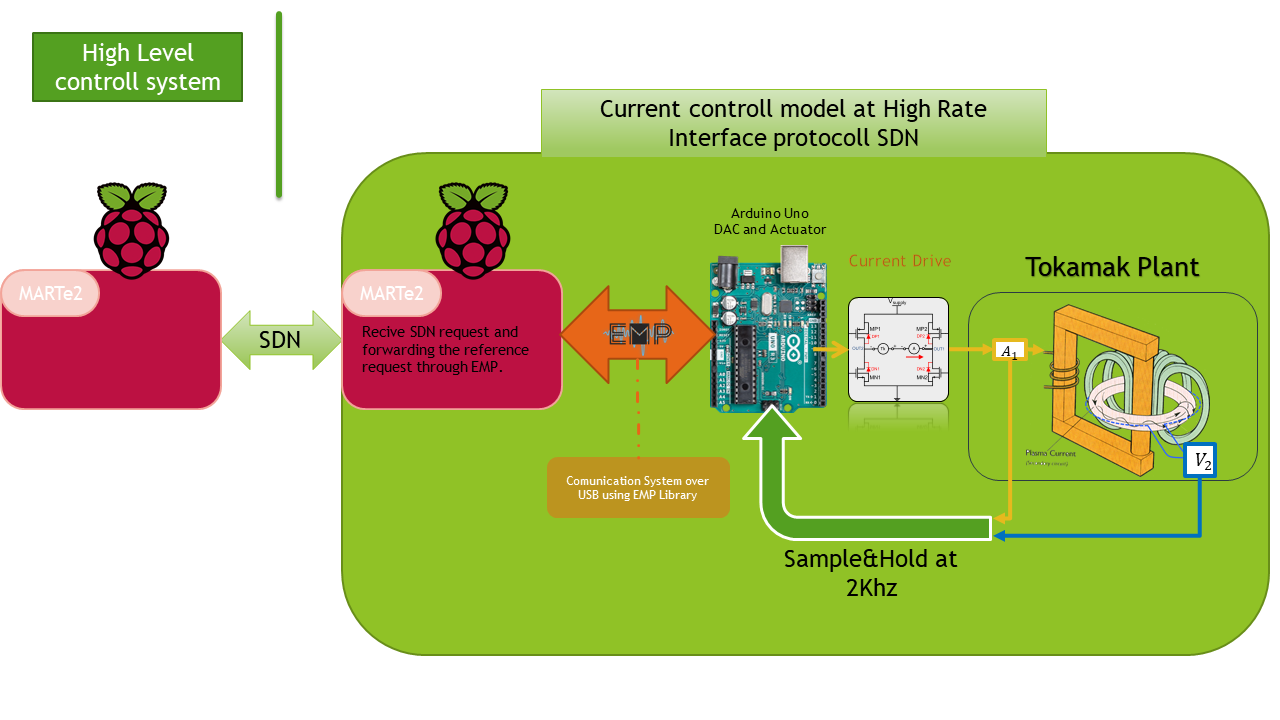
\includegraphics[width=1\textwidth]{Architettura/SystemArchitetture.png}
	\caption[Schema finale dell'archiettettura di controllo]{Architettura di controllo}
\end{figure}

\noindent
Lo schema proposto realizza l'obiettivo è controllare una singola bobina, il progetto finale prevederà la ripetizione in serie del medesimo schema per il numero di bobine necessarie.\\

Dallo schema risulta evidente che tutti i componenti visti nel capitolo "\nameref{cap:1}" si relazionano con lo stesso \microControllore: l'\ArduinoUno.\\
Per riportare i dati fuori e ricevere il riferimento da inseguire nella $V_2$, è stata realizzato il \nameref{EMP}, essa è stata scritta in C++ affinché possa essere Cross-Platform.\\
Il suo compito specifico, in questo progetto, è di mettere in comunicazione l'\ArduinoUno con un nodo \MARTe installato su di una \Rasp.\\
Quest'ultimo nodo ha il compito di mettere in rete il feedback dell'esperimento, e comunicare all'\ArduinoUno eventuali cambio di riferimento. Questo ultimo tratto è realizzato mediante il protocollo \textbf{SDN}, che viaggia sopra Ethernet e dà garanzie Real-time.\\
Nella sua forma finale, il progetto prevede la riproduzione in serie di questo schema di controllo per arrivare a controllare tutte le bobine poloidali presenti in un tokamak.

\newpage

\section*{EMP - Libreria di Comunicazione Seriale\\Embedded Message Pack }\label{sec:EMP}
\addcontentsline{toc}{section}{\protect\numberline{\thesection} EMP - Libreria di Comunicazione Seriale}

\begin{figure}[h]
	\centering
	
\includegraphics[width=1\textwidth]{EMP/EMP-Logo-Background.png}
\end{figure}
\paragraph{\citefield{EMP}{title}} nasce con l’obiettivo di standardizzare un protocollo e creare una libreria C++ basata su classi Template, che permetta di automatizzare e standardizzare tutto il lavoro di programmazione necessario all’invio/ricezione di dei pacchetti dal formato Pre-Concordati tra 2 Device connessi Peer2Peer (Nessuna pretesa di network-ing). (\cite{EMP})\\
Il raggiungimento dei suoi obiettivi, si sposa con la possibilità di supportare altre features interessanti:

\paragraph{Multiple-Package} Il protocollo di comunicazione che si è deciso di usare per EMP ha permesso di estendere il suo funzionamento e permettere il trasporto, attraverso lo stesso mezzo, di \textit{\textbf{pacchetti di tipologia e dimensione diversa}} all’interno della stessa libreria, evitando al contempo di inviare per ogni pacchetto più byte di quelli strettamente necessario. $\Rightarrow$ \textbf{Alta Efficienza}

\paragraph{Zero Tempo di negoziazione} Sempre grazie al protocollo di comunicazione, EMP è adatto ad un uso ‘Streaming’, questo perché non è necessario alcuna fase di sincronizzazione iniziale o durante la trasmissione in caso di perdita di dati, in aggiunta a ciò, EMP è in grado di scartare pacchetti errati in maniera trasparente all’utilizzatore. Tutto questo grazie al protocollo che \textbf{Auto-delimita i singoli pacchetti}. $\Rightarrow$ \textbf{Trasparenza Totale}

\paragraph{Responsabilità} Le uniche responsabilità a carico degli utilizzatori sono il riempimento dei pacchetti e la definizione degli stessi tra i 2 estremi della comunicazione.

\subsection*{Consistent Overhead Byte Stuffing (COBS)}
\addcontentsline{toc}{section}{\protect\numberline{\thesection} Protocollo - COBS}
Il protocollo di comunicazione che permette l’invio di \textbf{pacchetti diversi} e \textbf{senza fasi di negoziazione} alla base della libreria è \textbf{COBS}(\cite{COBS}).\\
Si tratta di un algoritmo per la codifica di byte, progettato per essere al tempo stesso efficiente e non ambiguo, che permette la definizione di \textit{data-pack frame} \textbf{Auto-delimiti} .

\begin{figure}[h]
	\centering
	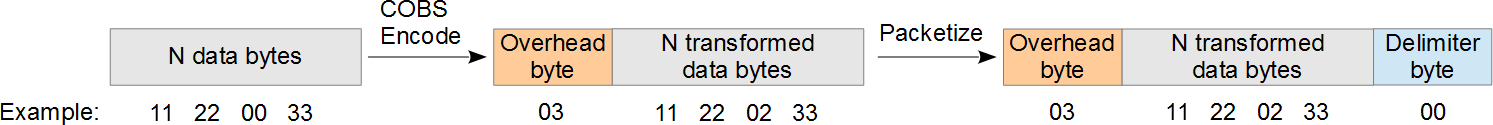
\includegraphics[width=1\textwidth]{EMP/Cobs_encoding_with_example.png}
	\caption[Esempio di COBS]{Esempio di COBS}
\end{figure}

\subsection{Metodo di codifica}
L'algoritmo di COBS trasforma una stringa arbitraria di byte, ciascuno dei quali ha un Range di valori da \textbf{[0:255]} in una nuova stringa di byte dove però ogni byte va da \textbf{[{\color{red}1}:255]}. La dimensione della nuova stringa è sempre pari alla dimensione della precedente + 1.\\
L'obiettivo di questo metodo di codifica è di eliminare tutti i possibili byte \zeroByte dal pacchetto in maniera reversibile.\\
Questo processo rende il carattere \textbf{\zeroByte (byte zero)} ottimo candidato per essere usato come terminatore di stringa durante l'invio, rendendo un pacchetto COBS-Encoded mai ambiguo e sempre \textbf{Auto-delimitato}.\\
L'algoritmo di codifica consiste nel:
\begin{enumerate} [itemsep=-3mm]
	\item Inserire un byte \zeroByte all'inizio del pacchetto
	\item Individuare tutti gli altri byte \zeroByte
	\item Inserire un byte \zeroByte alla fine del pacchetto
	\item Sostituire tutti gli \zeroByte con la distanza dal successivo \zeroByte nella stringa, ignorando l'ultimo
\end{enumerate}

\begin{figure}[h]
	\centering
	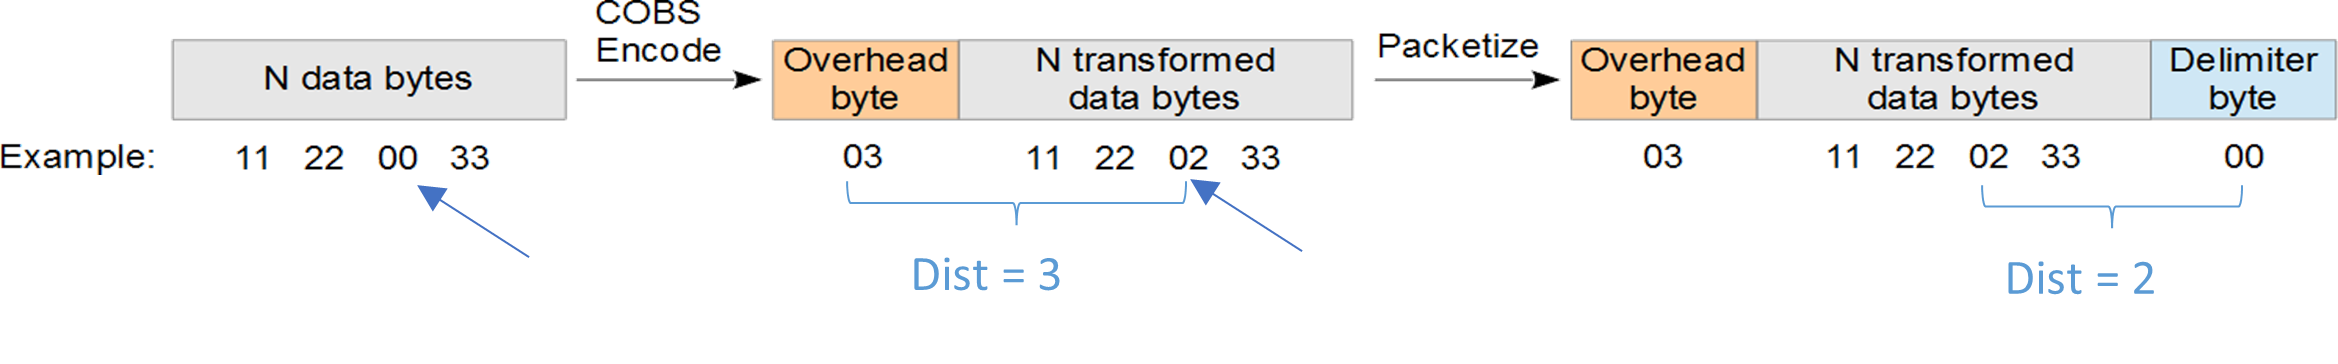
\includegraphics[width=1\textwidth]{EMP/Cobs_encoding_with_example-dist.png}
	\caption[Esempio di COBS con distanza]{Esempio di COBS con distanza}
\end{figure}

La versione usata per questo progetto, che comunque non ha l'obiettivo di trasmettere quantità infinite di byte, ha il limite di non poter codificare blocchi di byte che hanno una distanza tra 2 \zeroByte superiore a 255, questo limite è potenzialmente rimovibile usando un algoritmo più sofisticato.

\subsection{Caratteristiche chiave}
Prima caratteristica vincente della libreria è il suo alto grado di adattabilità, essa infatti per poter funzionare richiede solo \textbf{2 informazioni critiche} (e altre di contorno per l'allocazione opportuna dei buffer), esse sono i tipi dei pacchetti in \textbf{ Input} (\textit{pIn}) e in \textbf{Output} (\textit{pOut}) ovvero sia delle strutture in C, con i dati organizzati in base al messaggio da trasferire (\nameref{lst:EMPpackDef}).\\
In secondo luogo, la codifica \citefield{COBS}{title}, che abbiamo appena visto permette di avere pacchetti \textbf{Auto-delimitati}, ciò permette quindi di scambiare pacchetti diversi tra loro (sia per tipologia che per lunghezza) lungo \textbf{lo stesso} \textit{Stream} di dati.\\
L'unica condizione neccessaria è che il destinatario sia capace di determinare la tipologia di contenuto trasportato nel pacchetto semplicemente leggendolo.\\
Questo può essere facilmente risolto in più modi:
\begin{spacing}{1.5}
	\begin{description}
		\item[Lunghezza Univoca] Ogni possibile pacchetto ha una lunghezza diversa da tutti gli altri, $\Rightarrow$ la lunghezza implica il contenuto
		\item[Aggiunta di un campo Tipologia] Aggiungendo al’inizio della trasmissione un \textit{type byte}, ovviamente Pre-Concordato, diventa possibile per chiunque sapere come interpretare il contenuto del pacchetto.
	\end{description}
\end{spacing}
\noindent
Il metodo più universale è sicuramente l'aggiunta di un campo fisso per il tipo, di cui un esempio è visibile nell'appendice al listato \ref{lst:EMPmultiplePack}. (\nameref{lst:EMPmultiplePack})

In ogni caso, la codifica \citefield{COBS}{title} aggiunge 2 byte extra al pacchetto che si vuole inviare, e tanto per la codifica quanto per la decodifica in ricezione, il \textbf{costo} è sempre pari a \textbf{O(n)}.

\begin{multicols}{2}
	\begin{center}
		{\large Vantaggi:}
	\end{center}
	\begin{spacing}{1.25}
		\begin{enumerate}[itemsep=-1mm]
			\item Pacchetti {\color{Azure}\textbf{Self-Delimited}}
			\item Canale {\color{Azure}\textbf{Multi-Packet ready}}
			\item Protocollo {\color{Azure}\textbf{Senza Negoziazioni}}
			\item All’utilizzatore è richiesto solo di Pre-Concordare il formato del pacchetto con l’altro lato dello stream
			\item Prerequisiti implementativi minimale (mezzo di comunicazione a bytes di tipo \textit{peer2peer} asincrono)
		\end{enumerate}
	\end{spacing}
	\vfill
	\columnbreak
	\begin{center}
		{\large Svantaggi:}
	\end{center}
	\begin{spacing}{1.25}
		\begin{enumerate}[itemsep=-1mm]
			\item Aggiunge 2 byte fissi
			\item Richiede O(n) elaborazione sia in codifica che decodifica
		\end{enumerate}
	\end{spacing}
	\vspace*{\fill}
\end{multicols}

\newpage

\subsection{Integrità dei pacchetti}
Per aumentare ulteriormente i campi d’uso e garantire un layer minimale di \textbf{integrità} sui pacchetti in transito, la libreria è stata progettata per include in maniera trasparente anche un un check di errore calcolato usando \cite{CRC8}, aggiunto in trasmissione e rimosso in ricezione.\\
L'aggiunta e il calcolo del CRC8 viene fatta sul pacchetto non ancora \textit{COBS-Encodato}, ciò garantisce la possibilità di inviare il pacchetto a prescindere da quale sia il risultato del CRC8, e viene quindi verificato dopo aver de-\textit{COBS-Encodato} il pacchetto in ricezione.\\
Questa features deve essere attiva o disattivata da entrambi i lati della libreria (ne consegue che anche lei deve essere pre-concordata tra i 2 estremi).\\
La libreria, se attiva, è in grado di capire se il pacchetto ha subito degli errori (ovviamente nei limiti del CRC8) e in tal caso scarta il pacchetto ricevuto in maniera totalmente trasparente all'utilizzatore.\\
L’aver usato COBS come sistema di codifica per la trasmissione, garantisce che la decodifica debba avvenire solo nei byte compresi tra 2 zeri, e se questa decodifica presenta un errore, toglie ogni ambiguità sul da farsi poiché il pacchetto viene scartato e si attende un successivo 0 mentre si memorizzano i byte ricevuti nel frattempo.

\newpage
\subsection{Struttura del codice}
Lo sviluppo del codice è qui riassunto nel \textbf{Class Diagram} fatto in UML, del codice:
\begin{figure}[h]
	\centering
	\includegraphics[width=1\textwidth]{EMP/EMP-Hierarchy.png}
	\caption[Class Diagram UML di EMP]{Class Diagram UML}
\end{figure}
\noindent
Senza entrare eccessivamente nel dettaglio di \citefield{EMP}{title}, poichè tutti i codici, esempi e lavori aggiornati, sono reperibili nel repositori di \cite*{EMP}, possiamo iniziare osservando che il codice è diviso in 2 macro blocchi (\textbf{MPCore}, \textbf{MP}) più una classe di supporto per il buffer circolare.\\
Questa organizzazione del codice è stata pensata per far compilare su tutte le piattaforme di interesse lo stesso codice attivo, presente in \textbf{MPCore}, mentre le particolarizzazioni dovute alle varie piattaforme o al mezzo di comunicazione sono demandate alle classi concrete che però, come si vede, discendono tutte dallo stesso padre.\\
Questo metodo di sviluppo ha minimizzato enormemente i tempi di sviluppo, poiché una volta testato il codice \textbf{Core} funzionante, non è rimasto che adattare i dettagli per estenderne l'ambiente di sviluppo. Con questa tecnica è virtualmente possibile estendere su qualsiasi piattaforma la libreria, avendo \textbf{MPCore} delle richieste per compilare estremamente esigue, senza troppe complicazioni, e, se la piattaforma lo concede come nel caso di Linux, raccogliere ulteriormente delle funzionalità comuni e scrivere così, via via, sempre meno codice.


\newpage
\subsection{Benchmark}

\newpage
\section{Online Sampling}
\subsection{Interconnessione Arduino $\Leftrightarrow$ Companion}
\subsection{Storage su file delle informazioni}

\newpage
\section{Post Elaborazione con Matlab}
\subsection{Conversioni Dati}
\subsection{Creazione dei grafici e Filtraggio}
